\chapter{Analiza dziedziny problemu}
W dzisiejszych czasach, przed firmami archeologicznymi stoi nie małe wyzwanie, polegające na przeprowadzaniu badań archeologicznych na coraz większych powierzchniowo obszarach. Przedinwestycyjne badania wykopaliskowe (w których specjalizuje się firma "JN-Profil" - docelowy użytkownik oprogramowania stworzonego w ramach niniejszej pracy) polegają na przeprowadzeniu badań terenowych oraz stworzeniu dokumentacji podsumowującej rezultaty tych badań.

Dokumentacja archeologiczna zawiera w sobie dużą liczbę dokumentów, z których co najmniej część opiera się na tych samych danych, których proces przetwarzania można, a nawet powinno się zautomatyzować. Do tej pory tworzenie dokumentacji sprowadzało się do mozolnego kopiowania danych z jednego miejsca do drugiego, jednak dzięki współcześnie dostępnym technologiom informatycznym istnieje możliwość zautomatyzowania i przyspieszenia tego procesu - co w szerszej perspektywie prowadzi do zmniejszenia kosztów przeprowadzania badań archeologicznych.

\section{Wymgagania biznesowe}
Przed systemem do prowadzenia ewidencji badań archeologicznych jest stawiany szereg wymagań, których spełnienie jest warunkiem poprawnego funkcjonowania oraz zadowolenia użytkowników. Część z nich jest wspólna dla wszystkich systemów informatycznych, natomiast reszta jest związana z charakterem pracy archeologa.

Aby system nadawał się do profesjonalnego użytku, konieczne jest, aby efekty pracy były zapisane w pamięci trwałej. Konieczne jest także, aby możliwe było równoległe korzystanie wielu użytkowników, z dodatkowym zastrzeżeniem, że równoległe sesje użytkowników mogą pracować na tych samych danych i system powinien mimo to gwarantować ich spójność.

Specyficzną cechą pracy archeologa jest konieczność wyjazdów i prowadzenia badań archeologicznych w różnych miejscach. System wspierający prowadzenie ewidencji badań archeologicznych powinien umożliwiać tworzenie dokumentacji z różnych miejsc i urządzeń. 
\newpage
\section{Słownik dziedziny problemu}
Na samym początku opracowywania systemu dla przedsiębiorstwa należy zdefiniować wszystkie elementy występujące w codziennej pracy, aby nie było wątpliwości co do zrozumienia tematu. 

\begin{itemize}
\item Obiekt - obiekt archeologiczny, główny cel badań. Obiekt to prawdopodobny ślad działalności człowieka, bardzo często jest postaci pozostałości po palenisku.
\item Zabytek wydzielony - zabytek większej wartości, dokumentowany i opisywany osobno. Na przykład - trzonek siekierki.
\item Zabytek masowy - kilka zabytków, zgrupowanych w pozycjach dokumentacji jako jeden. Zazwyczaj składa się z niewielkich przedmiotów, np. krzemień czy ceramika o wielkości kilku centymetrów kwadratowych
\item Rysunek - sposób dokumentowania zabytków i obiektów. Zazwyczaj rysunek przedstawia rzut albo profil obiektu lub obrys zabytku.
\item Zdjecie - sposób dokumentowania obiektów, rzadziej zabytków. Najczęściej powstają w trakcie eksploracji obiektów, tj zaraz po odsłonięciu obiektu (zdjęcie rzutu), następnie po wyeksplorowaniu połowy (profil) i na końcu zdjęcie wyeksplorowanego obiektu (negatyw).
\item Ar - jednostka powierzchni wykopalisk archeologicznych. Punkt odniesienia dla wszelkich informacji w dokumentacji.
\item Typ zabytku - Podział zabytków (masowych) ze względu na typ zabytku. Klasyfikacja najczęściej pojawiających się zabytków, np. fr. ceramiki, okruch (Krzemienia)
\item Grupa zabytków - Bardzo ogólny podział zabytku, zazwyczaj podział jest na trzy grupy (Ceramika, Krzemień, Inne)
\item Profil - przekrój wyeksploatowanego obiektu, jeden z dokumentowanych elementów
\item Rzut - widok obiektu z góry, przed eksploatacją
\item Calec - rodzaj otoczenia znajdującego się dookoła obiektu, jednak nie będący nim, np. less.
\item Kultura - zespół stale współwystępujących ze sobą na pewnym terytorium i w pewnym czasie charakterystycznych form źródeł archeologicznych.
\item Funkcja - określona w ramach badań obiektu jego obecność i przyczyna jego powstania
\item Chronologia - pozwala na określenie wieku znaleziska
\item Eksploracja obiektu - proces badania obiektu archeologicznego polegająca na wydobyciu jego zawartości w miedzyczasie udokumentowując kolejne etapy wykonywania badania
\end{itemize}
\newpage
\section{Model dziedziny problemu}
W systemie wspierającym działalność firmy archeologicznej powinno się wyróżnić 6 najważniejszych elementów (opisanych w poprzednim podrozdziale):
\begin{itemize}
\item Zabytki Masowe\\
\item Zabytki Wydzielone\\
\item Obiekty Archeologiczne\\
\item Zdjęcia\\
\item Rysunki\\
\item Ary
\end{itemize}

Wszystkie powyższe obiekty są produktem przeprowadzanego badania archeologicznego, dlatego są bytami, które mają sens tylko w konkretnym kontekście biznesowym (czyli opracowaniu). Wszystkie inne informacje wprowadzone do systemu są uniwersalne dla badań archeologicznych, dlatego są dostępne i edytowalne niezależnie od opracowania.

\begin{figure} [H]
    \begin{center}
	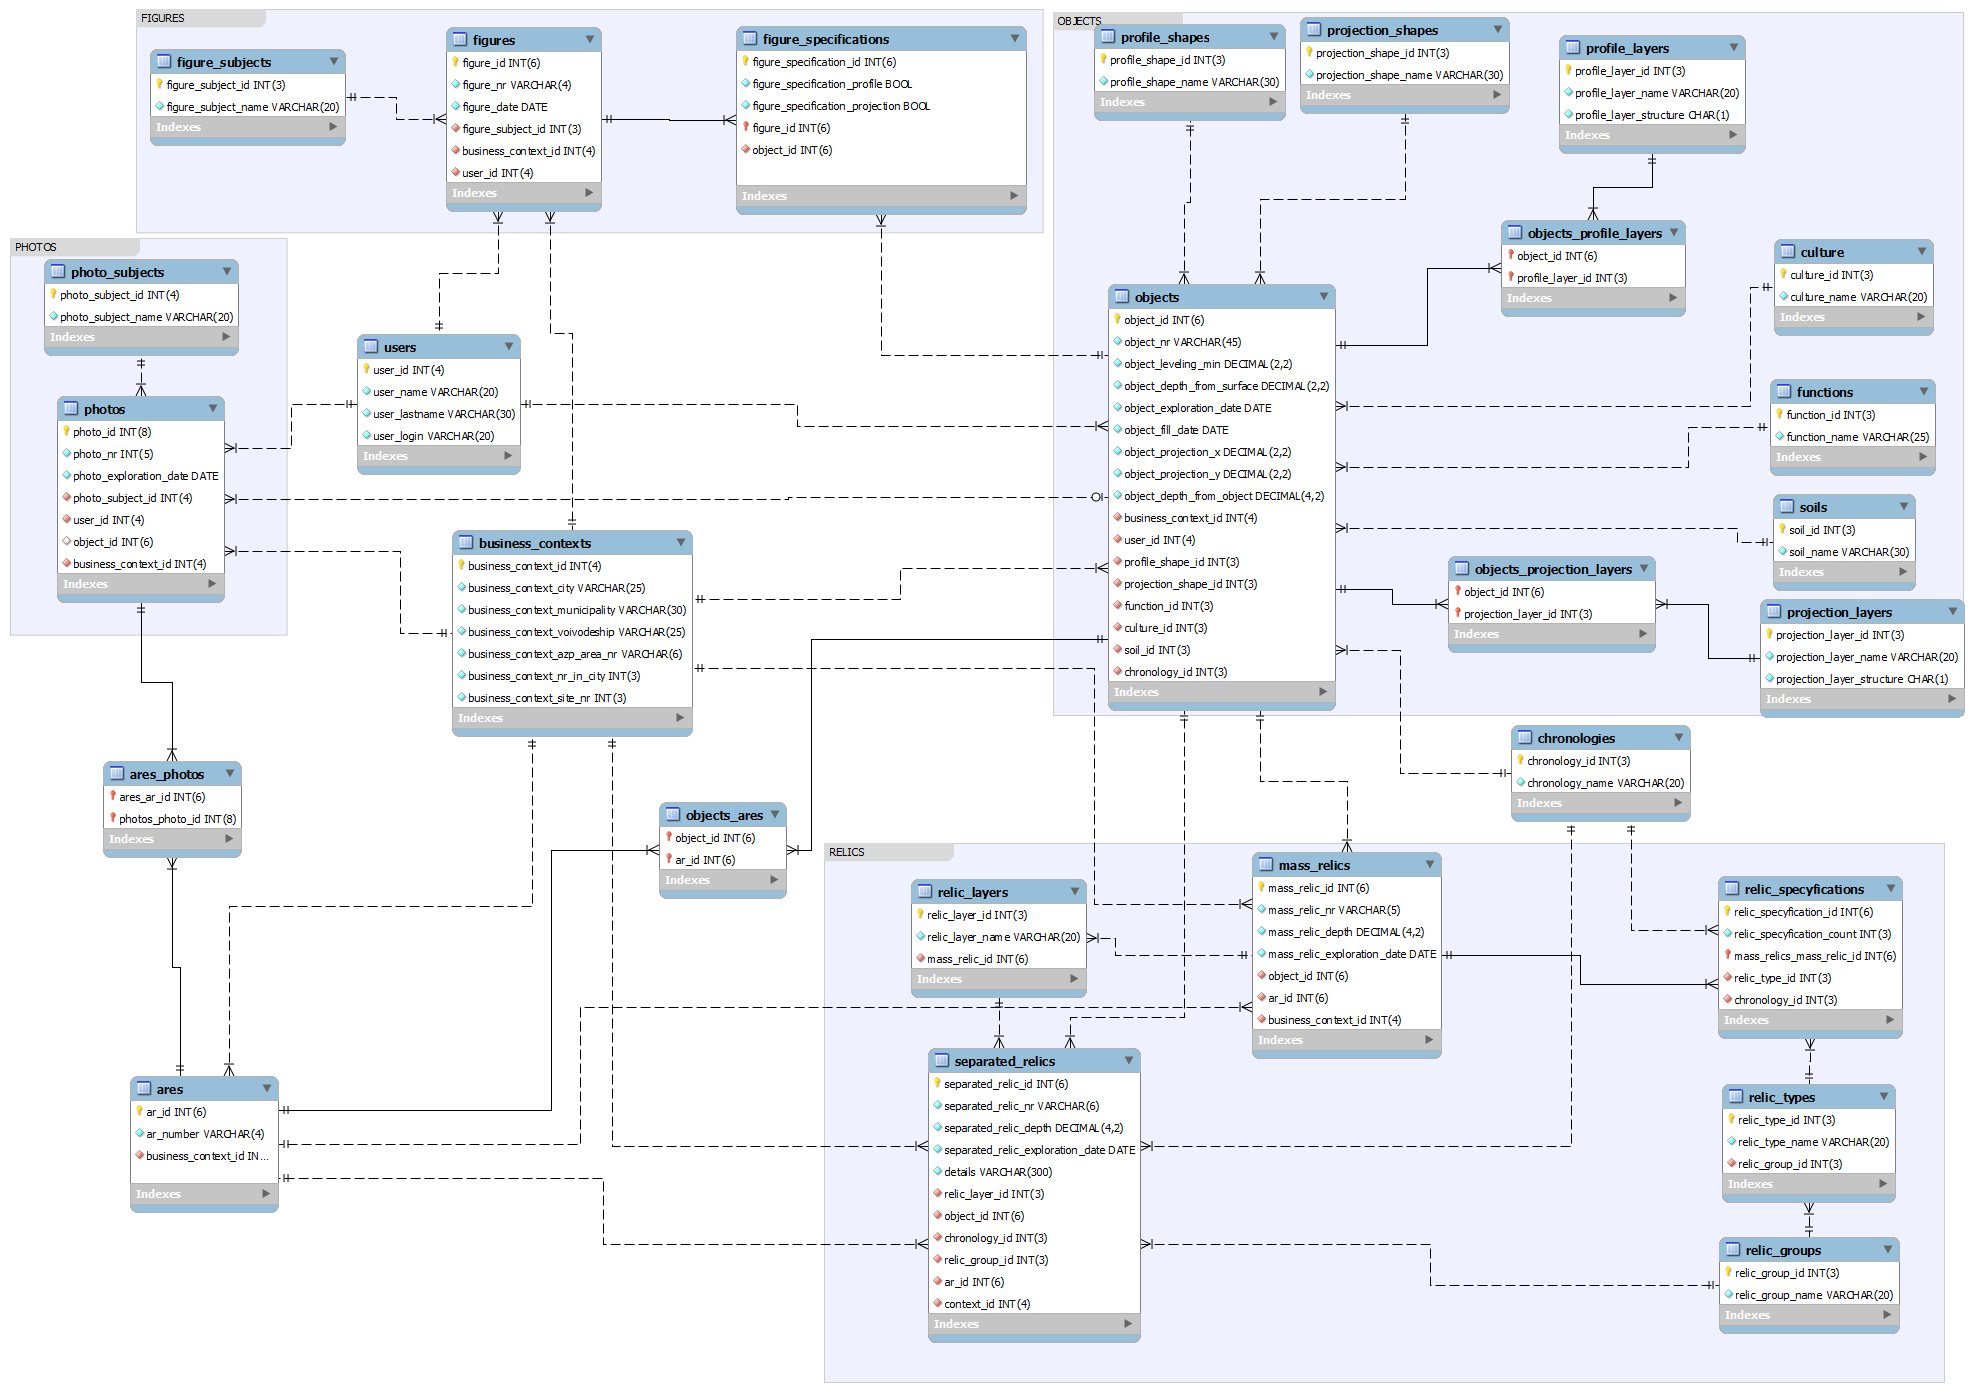
\includegraphics[angle=90, scale=.26]{img/db.png}
	\caption{Model dziedziny}
	\label{modelDziedziny}
    \end{center}
\end{figure}

Jak widać, poza głownymi elementami bazy danych odpowiadającym elementom specyficznym dla badania występuje duża ilość encji słownikowych, co powoduje znaczne zwiększenie koniecznego nakładu pracy. 
\newpage
\section{Model przypadków użycia}
Zadaniem systemu wspierającego tworzenie dokumentacji archeologicznej powinno być umożliwienie wprowadzenia danych w łatwy i przejrzysty sposób oraz szybkie generowanie raportów, będących składnikami dokumentacji archeologicznej.

\begin{figure} [H]
    \begin{center}
	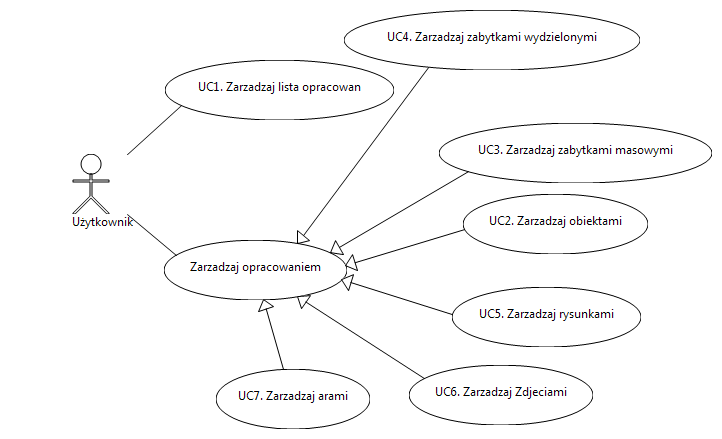
\includegraphics[scale=.5]{img/useCaseZarzadzanieOpracowaniem.png}
	\caption{Diagram przypadków użycia dla obiektów specyficznych dla opracowania}
	\label{useCasesDiag1}
    \end{center}
\end{figure}

Dodatkową cechą systemu będącego produktem niniejszej pracy jest to, że możliwa jest edycja słowników służących do wypełniania danych z poziomu okna edycji obiektu wypełnianego.
\newpage
\begin{figure} [H]
    \begin{center}
	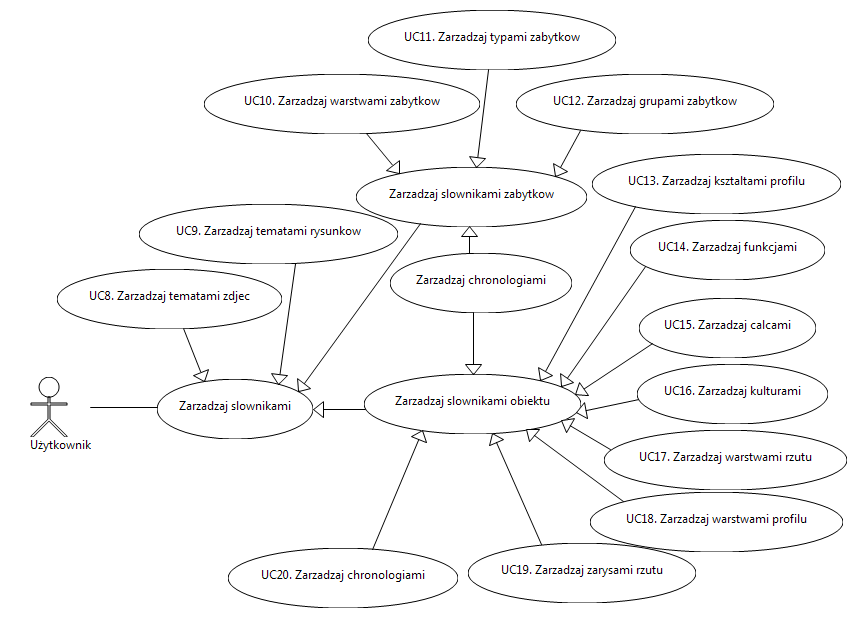
\includegraphics[scale=.5]{img/useCasesZarzadzanieSlownikami.png}
	\caption{Diagram przypadków użycia dla obiektów uniwersalnych względem opracowania}
	\label{useCasesDiag2}
    \end{center}
\end{figure}

Jak można zauważyć na podstawie diagramów przypadków użycia, każdy użytkownik ma takie same uprawnienia - tzn. może zarówno zarządzać listą opracowań, jak i modyfikować istniejące opracowanie, a także może edytować zawartość słowników.

% ex: set tabstop=4 shiftwidth=4 softtabstop=4 noexpandtab fileformat=unix filetype=tex spelllang=pl,en spell: